\documentclass[11pt,a4paper,openany]{book}

%\usepackage[german]{babel}	%in case you want to write a german thesis

%settings for generation of titlepage, index and table of content
\include{sections/Settings}

%definitions for easier costumization
\def \subtitle {Robot Extensible Communication Toolkit}
\def \year {2023/24}
\def \authors { \parseauthor{Projektmanagement. Rust Implementierung vom TCP/UDP und BLE Kommunikation. Performance Optimierungen für die Kommunikation}{Jeremy Sztavinovszki}{5CHIF}\\
                \parseauthor{Implementierung einer Rust gRPC Schnittstelle und das Eintragen einer Config in eine In-Memory SQLiteDB}{Christoph Fellner}{5BHIF} \\
				\parseauthor{Implementierung eines C++ Wrappers um die definierten gRPC Calls}{Maximilian Dragosits}{5CHIF} \\
				\parseauthor{Implementierung eines Tools und des Python Wrappers um die definierten gRPC Calls}{Timon Koch}{5CHIF} }
\def \supervisor { Harald Haberstroh }
\def \declauthors{ Jeremy Sztavinovszki, Christoph Fellner}	
\def \declauthors{ Timon Koch & Maximilian Dragosits}
% \def \declauthors{ Vor- und NACHNAME & Vor- und NACHNAME \\ Vor- und NACHNAME}	% for three authors

\addbibresource{main.bib}

\begin{document}
	%include titlepage
	\input{sections/titlepage}
	
	%include acknowledgements, abstract and documentation
	
	\pagestyle{plain}
	
	\frontmatter
	
	\pagenumbering{roman}
	\input{sections/declarationof}
	
	\tableofcontents
	
	\chapter{Acknowledgement}

The authors would like to thank their respective families, the HTBLuVA and robo4you 
for their support throughout the process of creating this diploma thesis. 

	

\chapter{Kurzfassung}

\textbf{Author: Sztavinovszki}

\vspace{10mm}

Eine der am meisten in der Robotik verwendeten Software Suiten ist das sogenannte Robot Operating System \footcite{ros-site} (kurz ROS).
Es ist eine Sammlung von Werkzeugen und Packeten, die verwendet werden, um hoch performante Robotik Systeme zu entwickeln und es abstrahiert
die Kommunikation zu Topics und Messages, die man in ROS-Bag Files aufzeichnen und abspielen kann. Das erlaubt es entwicklern sich auf die tatsächlichen Probleme der Entwicklung zu konzentrieren und sich nicht darum kümmern zu müssen Kommunikation neu zu implementieren.
ROS erlaubt außerdem die simulation Zahlreicher Komponenten von Robotern, welche man meistens als Digitale Zwillinge bezeichnet.
Einer der größten Nachteile, die ROS mit sich bringt ist die Komplexität und der Eigensinn, bei der Entwicklung. Diese Komplexität führt außerdem zu Performance einbußen, welche vor allem die Verwendbarkeit auf weniger Leistungsstarken Geräten, wie zum Beispiel dem KIPR Wombat Controller \footcite{wombat-controller}, welcher bei Schülern wegen seiner Kostengünstigkeit und Verwendbarkeit zum Einsatz kommt.

\medskip

Diese Arbeit wird erkunden, wie man eine Software ähnlich zu ROS implementiert. Es werden Probleme, wie zum Beispiel Inter Prozess Kommunikation \footcite{ipc-begriff}, Kommunikation durch Bluetooth Low Energy (BLE), TCP und UDP, und die Implementation von Kommunikations Libraries für verschiedene Programmiersprachen


\chapter{Abstract}

\textbf{Author: Sztavinovszki}

\vspace{10mm}


% Context or background information; general topic; specific topic.
In robotics one of the most important topics over the last couple of years has been communication. Communication doesn't only concern a robot being remote controllable. Mimimi keine Ahnung. 

% central questions or problem statement

% what's already known, what previous research has shown

% main reasons, rationale, goal for research

% research and or analytical methods

% main findings, results or arguments

% significance or implications


	
	%include thesis
	
	\mainmatter
	\pagenumbering{arabic}
	
	\chapter{Introduction}


\vspace{2mm}

\section{Motivation}
\textbf{Author: Sztavinovszki}
In almost every robotics application nowadays you need some kind of communication. Wether it is a robot communicating
its data to a home-base, or two robots sharing data with one another. Over the past years communication has drastically
improved with new protocols and technology, such as Bluetooth Low energy.

\section{Goal}
\textbf{Author: Sztavinovszki}

\section{History}

\section{Project Management}
\textbf{Author: Sztavinovszki}

\section{Outline}
%\section{Section}
%More text. \lipsum[1] See Figure~\ref{pic:example}.

%\begin{figure}[h]
%	\centering
%	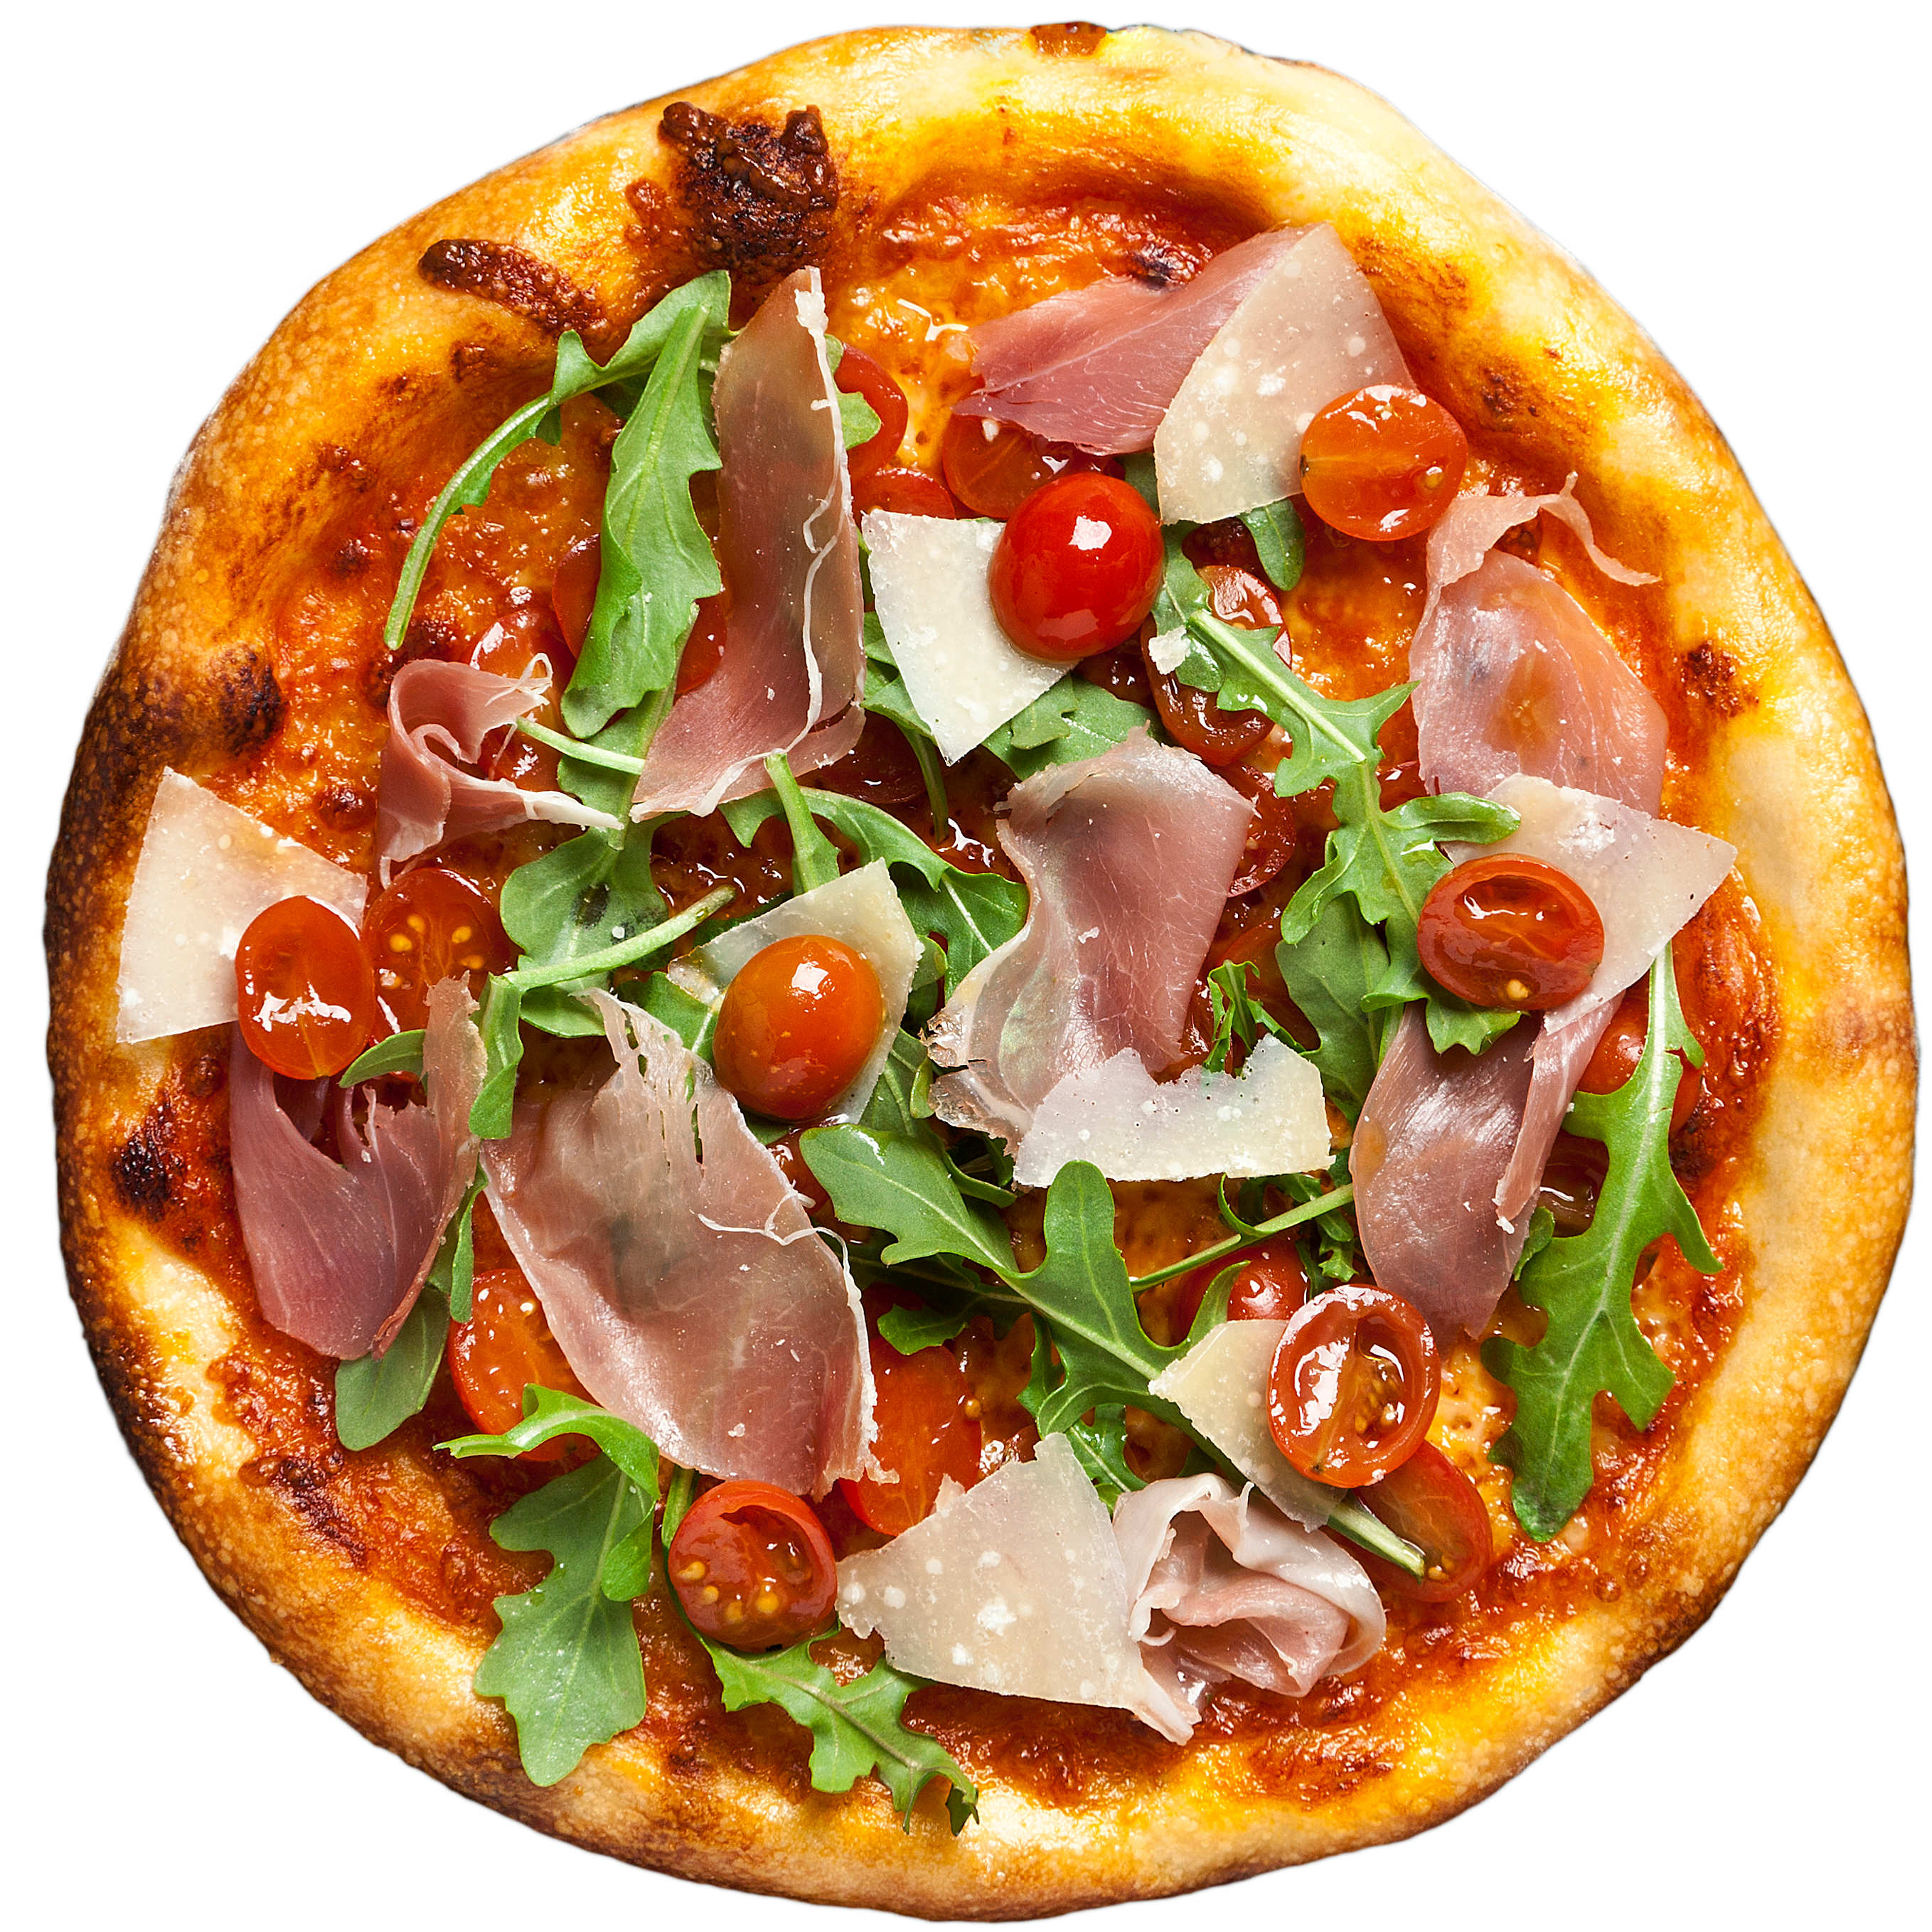
\includegraphics[width=2.5in]{img/example.png}
%	\caption{Picture description.}
%	\label{pic:example}
%\end{figure}

%\subsection{Subsection}
%\lipsum[1]

%\subsection{Subsection}
%\lipsum[1] See Table~\ref{tab:example}.

%\begin{center}
%	\begin{tabular}{| l | l | l |}
%		\hline
%		\bfseries Header 1 & \bfseries Header 2 & \bfseries Header 2 \\
%		\hline
%		Text & text & text \\
%		\hline
%		Text & text & text  \\
%		\hline
%		Text & text & text  \\
%		\hline
%	\end{tabular}
%	\label{tab:example}
%\end{center}

%\lipsum[1] Some references can be found at \footcite{robo4you} or at \footcite{Hope_Learning_TensorFlow}.
%

\filbreak

	\chapter{Study of Literature Sztavinovszki}

\textbf{Author: Jeremy Sztavinovszki} 

\section{The Rust Book}
% summary and main takeaway


\section{Network Programming with Rust}
% summary and main takeaway



\section{Main Takeaways}

\section{Getting Started with Bluetooth Low Energy}
Getting Started with Bluetooth Low Energy\footcite{ble_book} is a book giving deep insight into
the inner workings of Bluetooth Low Energy. The first four chapters are especially useful to this
work and are summed up in the following sections.

\subsection{Chapter 1. Introduction}
The introduction explains the history of Bluetooth Low
Energy from its start as Wibree, over the adoption by the Bluetooth Special Interest Group, to
the status at the time of the writing of the book. The chapter then goes on to explain the difference
to Bluetooth Classic. Key Limitations like Data througput and Operation range as well as possible network
topologies and the difference of Protocols versus profiles are also explained.  

\subsection{Chapter 2. Protocol Basics}
The second chapter goes over the different layers and protocols of Bluetooth Low Energy explaining the importance
and use for each of the layers and also covering the Generic Attribute Profile and the Generic Access Profile. It
provides explanations for the frequency hopping and modulation done in the physical layer and many other specifics
in the other layers.

\subsection{Chapter 3. GAP(Advertising and Connections)}
The third chapter explains concepts like roles, such as Broadcaster and Observer, and explains how each of them work.
It gives explanations of the modules and procedures included in the General Access Profile. After that section the Security
Manager and General Security constructs, such as Address Types, Authentication and Security Modes are covered. Lastly the GAP
service and the format in which data is sent over advertisements is covered.

\subsection{Chapter 4. GATT(Services and Characteristics)}
This chapter goes on to explain the roles defined in the Generall Attribute Profile and covers UUIDs.
Then the most important concept, Attributes, are explained. This chapter along with the documentation for the library this work uses for BLE solidified, that L2CAP is more suitable for this work. 
% Bla bla bla. Hier weiter schreiben.

\subsection{The Remaining Chapters}
The remaining covers go over specific hardware platforms, debugging tools, application design tools and platform specific mobile
programming and were not as important as the previous four chapters. Therefore they are not covered here.

\subsection{Main Takeaways}
The book provides great explanations of many difficult topics through text as well as visual aids. The main takeaways for this work are, that L2CAP is better suited for its purposes and better general knowledge of the BLE and its stack.


\filbreak

	\input{sections/methodology}
	\chapter{Implementation}

\section{CommLib}
\textbf{Author: Jeremy Sztavinovszki} 
The Communication Library, or CommLib for short is the part of the RECT stack, that handles all of the communication between the hosts over traditional protocols, like TCP, UDP and BLE.
This requires it to be especially performant. In order to avoid premature optimization however, the first part of this section on the implementation of the CommLib will only cover the first versions
of the code written to get the Library to work. After the first implementation there will be benchmarks and some profiling, in order to get a grasp on which aspects of the library need to be
optimized. The second section will then cover how these results were incorperated into designing a more polished version of the CommLib.

\subsection{Setting up the Library} 
The first steps of setting up the library are more or less the same as in any other rust project. First the project is initialized with \verb+cargo new --lib <rust-name>+. This creates a
new folder with the name specified in \verb+<library-name>+ and generates some files like Cargo.toml and src/main.rs. After this step is done the needed libraries for RECT are added to the
project through \verb+cargo add <dependency-name> -F <dependency-name>/<feature-name>+ these dependencies are the pulled and built by cargo (Rust's build tool) upon the initial build of the
project. The first iteration of the project then had the following dependencies:

\begin{itemize}
	\item{tokio}
	\item{bluer}
	\item{anyhow}
\end{itemize}

All in all the commands used to generate the CommLib project and install all dependencies looked like this:
\newline
\begin{minipage}{\textwidth}
	\begin{lstlisting}[language=bash, caption=Setup Commands for CommLib]
		cargo new --lib comm_lib && cd comm_lib
		cargo add tokio bluer anyhow -F tokio/full,bluer/full
		cargo build
	\end{lstlisting}
\end{minipage}

\subsection{First Implementation}
The first part of the implementation that was tackled was to create an abstraction layer over the existing protocols that RECT uses.
in order to have a nice and clean interface to work with and to avoid having to implement each feature separately for the
protocols. Of course, there was a bit of a problem with UDP because it is not meant to send structured data, so there is no feature parity between TCP and BLE.
between TCP and BLE and UDP in this respect, and UDP is only used to send unstructured data streams. To encapsulate the structured and unstructured data sent over the
and unstructured data sent over the common interface, there needs to be a way to convert the data, whether structured or not, into and from bytes in a way that is performant and has minimal overhead.
and has minimal overhead. In order to meet the above requirements, the following structure has been implemented.
 
\subsubsection{Messages and Packets}
% TODO Write about the packets and messages and maybe do a nice graphic.
% TODO find cite for TCP and UDP MTU 
The first thing taken into consideration for designing a data and class structure that is able to be sent over all of the protocols is the MTU's of the different protocols. 
For TCP and UDP the MTU, or maximum transmission unit, is defined by the Maximum Segment Size Option (MSS), which is technically limited to 65535 bytes (64KB), but as defined
in RFC 2675 \footcite{rfc2675} an MSS value of 65535 is defined to be interpreted as infinity and to be determined by Path MTU Discovery \footcite{rfc9293}. For BLE the MTU is 
defined by the L2CAP and can be anywhere from 23 to 65535, but the packet is fragmented and recombined by the L2CAP for transmission, which practically makes it infinite. % TODO find out why ble book cant be cited 

Another requirement for the interface was to be able to encapsulate the mechanism of sending a request to a peer and receiving a response. 
To do this, a pair of messages was implemented. This pair of messages, aptly named Request and Response, contains the data needed to make this work. This means 
that the request contains information about what topic to call on the remote machine, the data needed to fulfil that call, and an identification of the calling process, 
while the response contains the returned data and the ID of the client to which it should be returned. This identification is used to avoid confusion as to which process the data should be returned to, 
for example, when multiple processes are requesting data from the same remote service.

The identification mechanism used in the above case of sending data to a single recipient can also be adapted to send messages to multiple recipients.
The only adaptation required for the requesting and responding application to be able to send and receive broadcasts is to create a proxy object on the receiving side that acts as a single 
receiver to receive the data for multiple connections and then forward that data to all subscribing processes.  

The last use case covered by comm\_ lib is the sending of a continuous stream of data. An example of this would be a sensor continuously sending data. To avoid the overhead of sending values over
protocols used in comm\_ lib, it was decided to require a separate interface, e.g. a socket, that is used only for streaming the described data. This means that when the receiving side
is establishing a connection, it only needs to look at the identifier, e.g. the IP address, of the connected peer to decide which process to pass the data to, instead of reading a connection 
name from the packet sent, minimising the size of the packets that need to be sent. 

% TODO Write about the connection manager and also program that stuff
\subsubsection{The ConnectionManager}
The most important component in the whole comm\_ lib is the ConnectionManager. It is a singleton object, which as the name would suggest manages all of the needed and used connections that are
requested by the client programs. Because the ConnectionManager is a singleton and because it must be able to handle being in concurrent execution environments the Rust borrow-checker has very
special requirements for how it is accessed. To meet these requirements the static variable holding the ConnectionManager singleton has needs to be wrapped in several objects to ensure it is
thread-safe, as well as making sure, that it is initialized and freed, when there are no references left to its smart-pointer. 

\begin{lstlisting}[language=Rust]
	pub static CONNECTION_MANAGER: Lazy<Arc<Mutex<ConnectionManager>>> =
	    Lazy::new(|| Arc::new(Mutex::new(ConnectionManager::new())));
\end{lstlisting}
Which leads to the above code, which has specifies, that the ConnectionManager is wrapped in the following types.

\begin{itemize}
	\item{Lazy. This type allows any object held by it to be initialized only once and only when it is first called upon}
	\item{Arc. Arc stands for atomic reference counter and is a type of smart-pointer used in rust, when pointers need to be thread safe}
	\item{Mutex. The mutex ensures, that only one process at a time can hold a reference to the held object in order to prevent issues such as race-conditions}
\end{itemize}

% TODO Pretend you didn't already make everything railway programming and it still crashes because of stupid things.

\subsection{Profiling and Benchmarking}

\subsection{Polishing}

\subsection{Documentation}

\section{Rust Service}
\subsection{Documentation}

\section{C++ Implementation}
\textbf{Author: Maximilian Dragosits}
The C++ Implementation is one of the two outward facing components of the RECT stack. Alongside the Python Implementation 
it serves as a library in order for developers to be able to create robots, that are able to communicate with each other, much
easier then before. This is accomplished by abstracting most of the complexities of gRPC behind the \textit{Rectcpp} class. 

The class only needs to be initialized with IP-Addresses for the different services that it offers and be given the IP of 
another of its kind and then it should be a simple act of using the predefined methods within the class in order to 
effortlessly communicate with other robots or devices running this or the Python frontend implementation.

\subsection{Rectcpp class}
\subsection{Documentation}

\section{Python Implementation}

\subsection{Documentation}

\section{Implementation Comparison}

\filbreak

	\chapter{Experiment 1}
\textbf{} 

\filbreak
	\input{sections/lessons_learned}
	\input{sections/experiment2}
	\chapter{Conclusion}

\textbf{Author: Jeremy Sztavinovszki} 
The previous sections of the thesis went over the goals, plans for using technologies and plans for combining the parts implemented in the thesis.
This section will go over the results of the thesis, revisit the goals and plans and give an outlook on what could be done in the future.

\section{Recap}
When starting the thesis, the goal was to create a system for robot communication that is extensible to any language and resource efficient. The system was based on gRPC for the communication between programs
and used Rust to communicate with peers over Bluetooth and WiFi. The plan was to implement two libraries in popular programming languages, one in Python and one in C++, that would implement a simple abstraction,
which allows for easy communication with the Rust service running in the background. Through these libraries the user would be able to send messages to other peers and receive responses, as well as sending streams to multiple
other peers. The Rust service would handle the communication with the peers and the user would not have to worry about the underlying communication protocol. The gRPC interface for the Rust service would keep a record of
the named connections, which users defined, in an in-memory database, which the underlying protocol would use to find the correct connection to send messages to.

\section{Results}
\subsection{The Python Library}
The Python library was implemented as planned and tested with a mock implementation of the Rust service. The library provides an easy to use interface for the user to send messages and streams to other peers and receive messages and streams back.
All functionality required for the library to work as discussed in the previous sections was realized.

\subsection{The C++ Library}
Sadly due to hardship encountered with the gRPC++ library, which is described in the previous sections, the C++ library did not get implemented fully. Everything except communicating over gRPC was designed and implemented.
This also means that the Rust service was not tested with the C++ library and no results regarding memory and CPU usage can be given at this point.

\subsection{The Rust Interface}
The Rust Interface, which handles the gRPC communication with other processes and manages the connections in the in-memory database, was implemented as planned. The interface was tested through tokio tests and mock clients and worked as expected.

\subsection{The Rust Communication Library}
Although the basic functionality of the Rust Communication Library(comm\_lib) was implemented, the library is unfinished. This is due to the complexity of the concurrency model. While the library can send and receive data over WiFi and
BLE the libraries higher level abstractions like sending messages and receiving acknowledgements, sending and receiving streams and sending and receiving requests and responses have not been implemented. This means, that neither the
Python Library, nor the Rust Interface could be tested for robot to robot communication.

\section{Outlook}
While some of the parts of the RECT stack were able to be finished others encountered problems, that lead to the team unable to fully finish the implementation during the time of the thesis.
Of course after such setbacks it is important to look at what could be done better in the future. Starting with the conception of the system, the team should have looked more into existing
systems and libraries and how they solve the problems encountered during the thesis. Furthermore a more detailed plan of how to do the communication between the parts of the system should have been made
before starting with the implementation and specification of the systems interface. This would have made it easier to see the problems with the gRPC++ library and the concurrency model of the comm\_lib.
Future work on the RECT stack should mainly focus on finishing the comm\_lib and the C++ library, as well as implementing more optimizations for the communication like doing compression of the data, which is sent over the network.
Furthermore implementing more programming language interfaces would be beneficial, as it would make the system more accessible to more users. Implementing interfaces for serial communication and other communication protocols would
also be beneficial, as it would make the system more versatile. Also while a system with fixed configurations like the one implemented in the thesis may be more efficient, a system for automatically discovering peers would be easier
to use, especially in a setting, where IP-Addresses and Ports are not known beforehand. For this reason implementing a DDS system similar to the one used in ROS would be a good idea. Finally after the system is finished it should
of course be tested under real conditions, like a competition.
% Get C++ library running
% Implement more optimizations
% Implement more programming language interfaces
% Implement abstractions for more communication protocols
% Implement a dds similar to ROS DDS'
% Try the system in real competitions

\filbreak
	
	
	% Index
	\newpage
	\chapter*{Index}
	\printindex[name]
	\printindex[title]
	
	\printbibliography
	
	\input{sections/messbox}

\end{document}
